\documentclass[12pt,ngerman,]{book}
\usepackage{lmodern}
\usepackage{amssymb,amsmath}
\usepackage{ifxetex,ifluatex}
\usepackage{fixltx2e} % provides \textsubscript
\ifnum 0\ifxetex 1\fi\ifluatex 1\fi=0 % if pdftex
  \usepackage[T1]{fontenc}
  \usepackage[utf8]{inputenc}
\else % if luatex or xelatex
  \ifxetex
    \usepackage{mathspec}
  \else
    \usepackage{fontspec}
  \fi
  \defaultfontfeatures{Ligatures=TeX,Scale=MatchLowercase}
\fi
% use upquote if available, for straight quotes in verbatim environments
\IfFileExists{upquote.sty}{\usepackage{upquote}}{}
% use microtype if available
\IfFileExists{microtype.sty}{%
\usepackage{microtype}
\UseMicrotypeSet[protrusion]{basicmath} % disable protrusion for tt fonts
}{}
\usepackage[margin=1in]{geometry}
\usepackage{hyperref}
\PassOptionsToPackage{usenames,dvipsnames}{color} % color is loaded by hyperref
\hypersetup{unicode=true,
            pdftitle={Praxis der Datenanalyse},
            pdfauthor={Sebastian Sauer, Matthias Gehrke, Karsten Lübke, Oliver Gansser},
            colorlinks=true,
            linkcolor=Maroon,
            citecolor=Blue,
            urlcolor=Blue,
            breaklinks=true}
\urlstyle{same}  % don't use monospace font for urls
\ifnum 0\ifxetex 1\fi\ifluatex 1\fi=0 % if pdftex
  \usepackage[shorthands=off,main=ngerman]{babel}
\else
  \usepackage{polyglossia}
  \setmainlanguage[]{german}
\fi
\usepackage{longtable,booktabs}
\usepackage{graphicx,grffile}
\makeatletter
\def\maxwidth{\ifdim\Gin@nat@width>\linewidth\linewidth\else\Gin@nat@width\fi}
\def\maxheight{\ifdim\Gin@nat@height>\textheight\textheight\else\Gin@nat@height\fi}
\makeatother
% Scale images if necessary, so that they will not overflow the page
% margins by default, and it is still possible to overwrite the defaults
% using explicit options in \includegraphics[width, height, ...]{}
\setkeys{Gin}{width=\maxwidth,height=\maxheight,keepaspectratio}
\IfFileExists{parskip.sty}{%
\usepackage{parskip}
}{% else
\setlength{\parindent}{0pt}
\setlength{\parskip}{6pt plus 2pt minus 1pt}
}
\setlength{\emergencystretch}{3em}  % prevent overfull lines
\providecommand{\tightlist}{%
  \setlength{\itemsep}{0pt}\setlength{\parskip}{0pt}}
\setcounter{secnumdepth}{5}
% Redefines (sub)paragraphs to behave more like sections
\ifx\paragraph\undefined\else
\let\oldparagraph\paragraph
\renewcommand{\paragraph}[1]{\oldparagraph{#1}\mbox{}}
\fi
\ifx\subparagraph\undefined\else
\let\oldsubparagraph\subparagraph
\renewcommand{\subparagraph}[1]{\oldsubparagraph{#1}\mbox{}}
\fi

%%% Use protect on footnotes to avoid problems with footnotes in titles
\let\rmarkdownfootnote\footnote%
\def\footnote{\protect\rmarkdownfootnote}

%%% Change title format to be more compact
\usepackage{titling}

% Create subtitle command for use in maketitle
\newcommand{\subtitle}[1]{
  \posttitle{
    \begin{center}\large#1\end{center}
    }
}

\setlength{\droptitle}{-2em}
  \title{Praxis der Datenanalyse}
  \pretitle{\vspace{\droptitle}\centering\huge}
  \posttitle{\par}
\subtitle{Skript zum Modul}
  \author{Sebastian Sauer, Matthias Gehrke, Karsten Lübke, Oliver Gansser}
  \preauthor{\centering\large\emph}
  \postauthor{\par}
  \predate{\centering\large\emph}
  \postdate{\par}
  \date{22 April, 2017}

\usepackage{booktabs}
\usepackage{longtable}
\usepackage[bf,singlelinecheck=off]{caption}

%\setmainfont[UprightFeatures={SmallCapsFont=AlegreyaSC-Regular}]{Alegreya}

\usepackage{framed,color}
\definecolor{shadecolor}{RGB}{248,248,248}

\renewcommand{\textfraction}{0.05}
\renewcommand{\topfraction}{0.8}
\renewcommand{\bottomfraction}{0.8}
\renewcommand{\floatpagefraction}{0.75}

%\renewenvironment{quote}{\begin{VF}}{\end{VF}}
\let\oldhref\href
\renewcommand{\href}[2]{#2\footnote{\url{#1}}}

\ifxetex
  \usepackage{letltxmacro}
  \setlength{\XeTeXLinkMargin}{1pt}
  \LetLtxMacro\SavedIncludeGraphics\includegraphics
  \def\includegraphics#1#{% #1 catches optional stuff (star/opt. arg.)
    \IncludeGraphicsAux{#1}%
  }%
  \newcommand*{\IncludeGraphicsAux}[2]{%
    \XeTeXLinkBox{%
      \SavedIncludeGraphics#1{#2}%
    }%
  }%
\fi

\renewcommand{\thesection}{\arabic{section}}  % ses




\makeatletter
\newenvironment{kframe}{%
\medskip{}
\setlength{\fboxsep}{.8em}
 \def\at@end@of@kframe{}%
 \ifinner\ifhmode%
  \def\at@end@of@kframe{\end{minipage}}%
  \begin{minipage}{\columnwidth}%
 \fi\fi%
 \def\FrameCommand##1{\hskip\@totalleftmargin \hskip-\fboxsep
 \colorbox{shadecolor}{##1}\hskip-\fboxsep
     % There is no \\@totalrightmargin, so:
     \hskip-\linewidth \hskip-\@totalleftmargin \hskip\columnwidth}%
 \MakeFramed {\advance\hsize-\width
   \@totalleftmargin\z@ \linewidth\hsize
   \@setminipage}}%
 {\par\unskip\endMakeFramed%
 \at@end@of@kframe}
\makeatother

\renewenvironment{Shaded}{\begin{kframe}}{\end{kframe}}

\newenvironment{rmdblock}[1]
  {
  \begin{itemize}
  \renewcommand{\labelitemi}{
    \raisebox{-.7\height}[0pt][0pt]{
      {\setkeys{Gin}{width=3em,keepaspectratio}\includegraphics{images/#1}}
    }
  }
  \setlength{\fboxsep}{1em}
  \begin{kframe}
  \item
  }
  {
  \end{kframe}
  \end{itemize}
  }
\newenvironment{rmdnote}
  {\begin{rmdblock}{note}}
  {\end{rmdblock}}
\newenvironment{rmdcaution}
  {\begin{rmdblock}{caution}}
  {\end{rmdblock}}
\newenvironment{rmdimportant}
  {\begin{rmdblock}{important}}
  {\end{rmdblock}}
\newenvironment{rmdtip}
  {\begin{rmdblock}{tip}}
  {\end{rmdblock}}
\newenvironment{rmdwarning}
  {\begin{rmdblock}{warning}}
  {\end{rmdblock}}
\newenvironment{rmdpseudocode}
  {\begin{rmdblock}{pseudocode}}
  {\end{rmdblock}}
\newenvironment{rmdexercises}
  {\begin{rmdblock}{exercises}}
  {\end{rmdblock}}
\newenvironment{rmdlove}
  {\begin{rmdblock}{love}}
  {\end{rmdblock}}

\usepackage{makeidx}
\makeindex

\urlstyle{tt}

\usepackage{amsthm}
\makeatletter
\def\thm@space@setup{%
  \thm@preskip=8pt plus 2pt minus 4pt
  \thm@postskip=\thm@preskip
}
\makeatother

\frontmatter

\begin{document}
\maketitle

{
\hypersetup{linkcolor=black}
\setcounter{tocdepth}{2}
\tableofcontents
}
\listoftables
\listoffigures
\section*{Vorwort}\label{vorwort}


\begin{center}
\includegraphics[width=0.3\linewidth]{images/FOM} \end{center}

Statistik heute; was ist das? Sicherlich haben sich die Schwerpunkte von
``gestern'' zu ``heute'' verschoben. Wenig überraschend spielt der
Computer eine immer größere Rolle; die Daten werden vielseitiger und
massiger. Entsprechend sind neue Verfahren nötig - und vorhanden, in
Teilen - um auf diese neue Situation einzugehen. Einige Verfahren werden
daher weniger wichtig, z.B. der p-Wert oder der t-Test. Allerdings wird
vielfach, zumeist, noch die Verfahren gelehrt und verwendet, die für die
erste Hälfte des 20. Jahrhunderts entwickelt wurden. Eine Zeit, in der
kleine Daten, ohne Hilfe von Computern und basierend auf einer kleinen
Theoriefamilie im Rampenlicht standen (Cobb
\protect\hyperlink{ref-cobb2007introductory}{2007}). Die Zeiten haben
sich geändert!

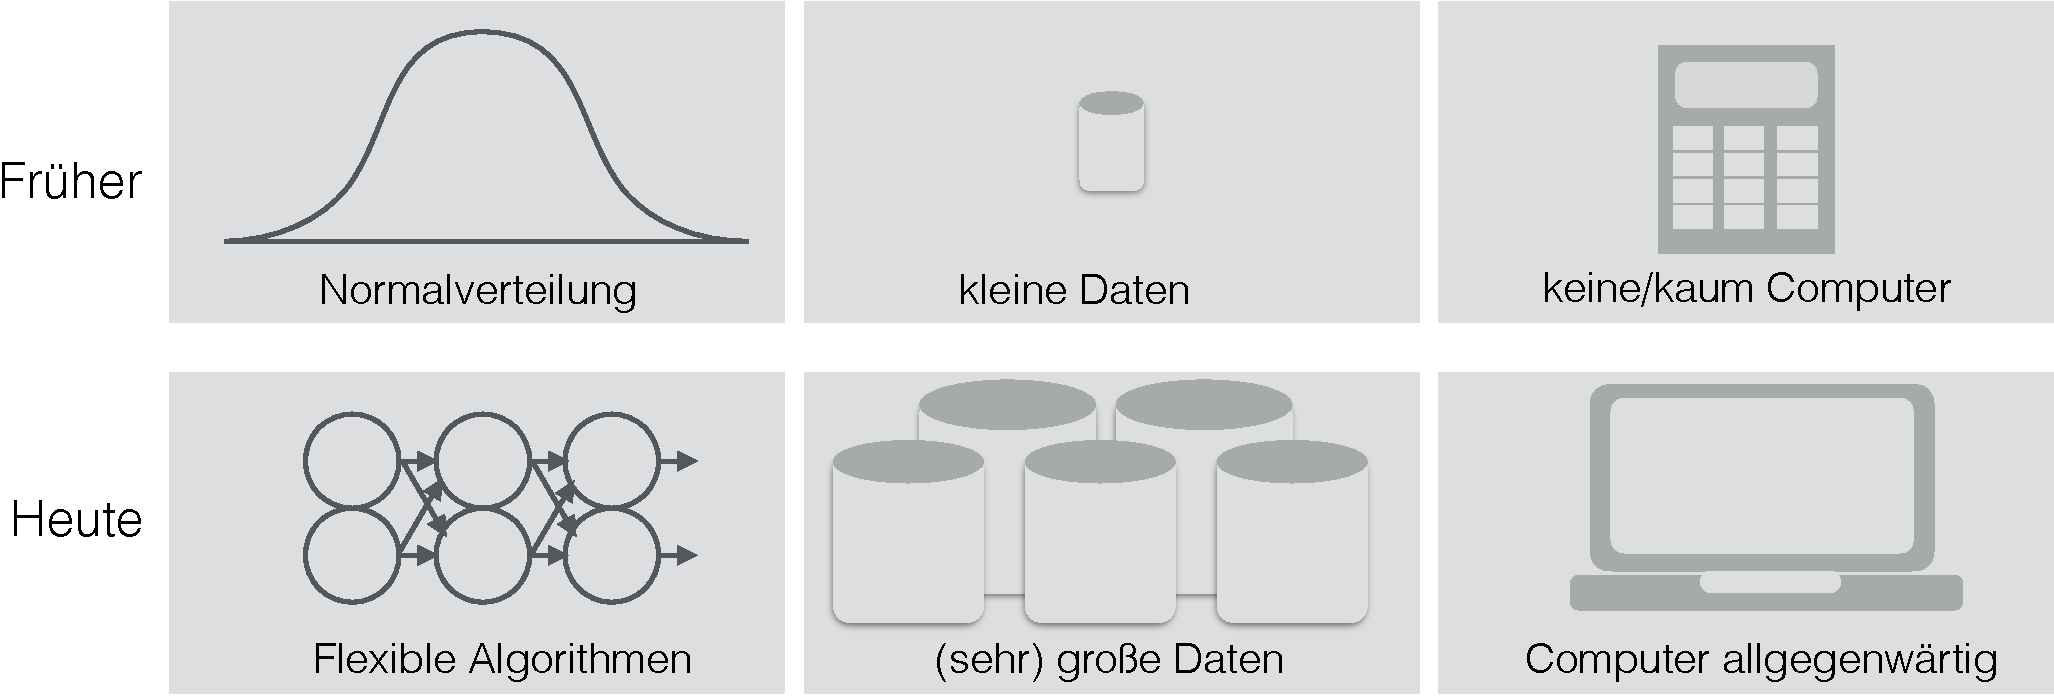
\includegraphics{images/Forschung_frueher_heute.pdf}

Zu Themen, die heute zu den dynamischten Gebieten der Datenanalyse
gehören, die aber früher keine große Rolle spielten, gehören (Hardin
u.~a. \protect\hyperlink{ref-hardin2015data}{2015}):

\begin{itemize}
\tightlist
\item
  Nutzung von Datenbanken und anderen Data Warehouses
\item
  Daten aus dem Internet automatisch einlesen (``scraping'')
\item
  Genanalysen mit Tausenden von Variablen
\item
  Gesichtserkennung
\end{itemize}

Sie werden in diesem Kurs einige praktische Aspekte der modernen
Datenanalyse lernen. Ziel ist es, Sie - in Grundzügen - mit der Art und
Weise vertraut zu machen, wie angewandte Statistik bei führenden
Organisationen und Praktikern verwendet wird\^{}{[}Statistiker, die
dabei als Vorbild Pate standen sind: Roger D. Peng:
\url{http://www.biostat.jhsph.edu/~rpeng/}, Hadley Wickham:
\url{http://hadley.nz}, Jennifer Bryan:
\url{https://github.com/jennybc}).

Es ist ein Grundlagenkurs; das didaktische Konzept beruht auf einem
induktiven, intuitiven Lehr-Lern-Ansatz. Formeln und mathematische
Hintergründe such man meist vergebens (tja).

Im Gegensatz zu anderen Statistik-Büchern steht hier die Umsetzung mit R
stark im Vordergrund. Dies hat pragmatische Gründe: Möchte man Daten
einer statistischen Analyse unterziehen, so muss man sie zumeist erst
aufbereiten; oft mühselig aufbereiten. Selten kann man den Luxus
genießen, einfach ``nur'', nach Herzenslust sozusagen, ein Feuerwerk an
multivariater Statistik abzubrennen. Zuvor gilt es, die Daten
aufzubereiten, umzuformen, zu prüfen und zusammenzufassen. Diesem Teil
ist hier recht ausführlich Rechnung getragen.

``Statistical thinking'' sollte, so eine verbreitete Idee, im Zentrum
oder als Ziel einer Statistik-Ausbildung stehen (Wild und Pfannkuch
\protect\hyperlink{ref-wild1999statistical}{1999}). Es ist die Hoffnung
der Autoren dieses Buches, dass das praktische Arbeiten (im Gegensatz zu
einer theoretischen Fokus) zur Entwicklung einer Kompetenz im
statistischen Denken beiträgt.

Außerdem spielt in diesem Kurs die Visualisierung von Daten eine große
Rolle. Zum einen könnte der Grund einfach sein, dass Diagramme
ansprechen und gefallen (einigen Menschen). Zum anderen bieten Diagramme
bei umfangreichen Daten Einsichten, die sonst leicht wortwörtlich
überersehen würden.

\begin{quote}
Dieser Kurs zielt auf die praktischen Aspekte der Analyse von Daten ab:
``wie mache ich es?''; mathematische und philosophische Hintergründe
werden vernachlässigt bzw. auf einschlägige Literatur verwiesen.
\end{quote}

\emph{R-Pseudo-Syntax}: R ist (momentan) die führende Umgebung für
Datenanalyse. Entsprechend zentral ist R in diesem Kurs. Zugebenermaßen
braucht es etwas Zeit, bis man ein paar Brocken ``Errisch'' spricht. Um
den Einstieg zu erleichern, ist Errisch auf Deutsch übersetzt an einigen
Stellen, wo mir dies besonders hilfreich erschien. Diese Stellen sind
mit diesem Symbol

\includegraphics[width=0.05000\textwidth]{images/pseudocode.png}
gekennzeichnet (für R-Pseudo-Syntax).

\emph{Achtung, Falle}: Schwierige oder fehlerträchtige Stellen sind mit
diesem Symbol

\includegraphics[width=0.05000\textwidth]{images/caution.png} markiert.

\emph{Übungsaufgaben}: Das Skript beinhaltet in jedem Kapitel
Übungsaufgaben oder/und Testfragen. Auf diese wird mit diesem Icon

\includegraphics[width=0.05000\textwidth]{images/exercises.png}
verwiesen oder die Übungen sind in einem Abschnitt mit einsichtigem
Titel zu finden.

\emph{Love}: Wenn Ihnen R diesen Smiley präsentiert, dann sind Sie am
Ziel Ihrer Träume:

\includegraphics[width=0.05000\textwidth]{images/love.png}.

Dieses Buch hat einige \emph{Voraussetzungen}, was das Vorwissen der
Leser angeht; folgende Themengebiete werden vorausgsetzt:

\begin{itemize}
\tightlist
\item
  Deskriptive Statistik
\item
  Grundlagen der Inferenzstatistik
\item
  Grundagen der Regressionsanalyse
\item
  Skalenniveaus
\item
  Grundlagen von R
\end{itemize}

Dieses Skript wurde mit dem Paket \texttt{bookdown} (Xie
\protect\hyperlink{ref-xie2015}{2015}) erstellt, welches wiederum stark
auf den Paketen \texttt{knitr} (Xie
\protect\hyperlink{ref-xie2015}{2015}) und \texttt{rmarkdown} (Allaire
u.~a.
\protect\hyperlink{ref-rmarkdown}{2016}\protect\hyperlink{ref-rmarkdown}{a})
beruht. Diese Pakete stellen verblüffende Funktionalität zur Verfügung
als freie Software (frei wie in Bier und frei wie in Freiheit).

Aus Gründen des Lesbarkeit wird das männliche Generikum verwendet,
welches Frauen und Männer in gleichen Maßen ansprechen soll.

Die Bildnachweise sind in folgenden Muster aufgebaut: Nummer, Verweis
zum Bild, Names des Autors, Titel, Quelle (URL), Lizenz, Abrufdatum.

\begin{enumerate}
\def\labelenumi{\arabic{enumi}.}
\item
  Abb. \ref{fig:modellieren-plot}, Sebastian Unrau, ohne Titel,
  \url{https://unsplash.com/photos/CoD2Q92UaEg}, CC0, 2017-02-12
\item
  Abb. \ref{fig:vwmodell}, Lothar Spurzem, VW 1303 von Wiking in 1:87;
  Größe des Modells: 47,5 mm,
  \url{https://de.wikipedia.org/wiki/Modellautomobil\#/media/File:Wiking-Modell_VW_1303_(um_1975).JPG},
  CC-BY-SA 2.0, de.
\end{enumerate}

Alle verwendeten Datensätze und R-Pakete finden sich im
Literaturverzeichnis; im Text werden Pakete nicht zitiert.

Ein Teil dieses Skripts basiert auf Arbeiten von meinen Kollegen Oliver
Gansser, Matthias Gehrke und Karsten Lübke. Ohne deren Unterstützung,
Ermutigung und Kritik gäbe es diesen Kurs nicht. Gerade von Karsten
Lübke habe ich einiges gelernt.

Sebastian Sauer

\section{Organisatorisches}\label{organisatorisches}

\section{Rahmen}\label{rahmen}

\section{Datenjudo}\label{datenjudo}

\section{Praxisprobleme der
Datenaufbereitung}\label{praxisprobleme-der-datenaufbereitung}

\section{Fallstudie zum Datenjudo}\label{fallstudie-zum-datenjudo}

\section{Daten visualisieren}\label{daten-visualisieren}

\section{Fallstudie zur
Visualisierung}\label{fallstudie-zur-visualisierung}

\section{Grundlagen des Modellierens}\label{mod1}

\section{Der p-Wert}\label{der-p-wert}

\section{Klassische lineare (numerische)
Regression}\label{klassische-lineare-numerische-regression}

\section{Klassifizierende Regression}\label{klassifizierende-regression}

\section{Fallstudien zum geleiteten
Modellieren}\label{fallstudien-zum-geleiteten-modellieren}

\section{nicht robust:}\label{nicht-robust}

\section{Vertiefung: Clusteranalyse}\label{vertiefung-clusteranalyse}

\section{Probeklausur}\label{probeklausur}

\section{Literaturverzeichnis}\label{literaturverzeichnis}

\hypertarget{refs}{}
\hypertarget{ref-rmarkdown}{}
Allaire, JJ, Joe Cheng, Yihui Xie, Jonathan McPherson, Winston Chang,
Jeff Allen, Hadley Wickham, Aron Atkins, und Rob Hyndman. 2016a.
\emph{rmarkdown: Dynamic Documents for R}.
\url{https://CRAN.R-project.org/package=rmarkdown}.

\hypertarget{ref-R-rmarkdown}{}
---------. 2016b. \emph{rmarkdown: Dynamic Documents for R}.
\url{https://CRAN.R-project.org/package=rmarkdown}.

\hypertarget{ref-R-gridExtra}{}
Auguie, Baptiste. 2016. \emph{gridExtra: Miscellaneous Functions for
„Grid`` Graphics}. \url{https://CRAN.R-project.org/package=gridExtra}.

\hypertarget{ref-R-BaylorEdPsych}{}
Beaujean, A. Alexander. 2012. \emph{BaylorEdPsych: R Package for Baylor
University Educational Psychology Quantitative Courses}.
\url{https://CRAN.R-project.org/package=BaylorEdPsych}.

\hypertarget{ref-R-quanteda}{}
Benoit, Kenneth, und Paul Nulty. 2016. \emph{quanteda: Quantitative
Analysis of Textual Data}.
\url{https://CRAN.R-project.org/package=quanteda}.

\hypertarget{ref-R-SnowballC}{}
Bouchet-Valat, Milan. 2014. \emph{SnowballC: Snowball stemmers based on
the C libstemmer UTF-8 library}.
\url{https://CRAN.R-project.org/package=SnowballC}.

\hypertarget{ref-breaking}{}
Briggs, William M. 2008. \emph{Breaking the Law of Averages: Real-Life
Probability and Statistics in Plain English}. Lulu.com.
\url{https://www.amazon.com/Breaking-Law-Averages-Probability-Statistics/dp/0557019907\%3FSubscriptionId\%3D0JYN1NVW651KCA56C102\%26tag\%3Dtechkie-20\%26linkCode\%3Dxm2\%26camp\%3D2025\%26creative\%3D165953\%26creativeASIN\%3D0557019907}.

\hypertarget{ref-uncertainty}{}
---------. 2016. \emph{Uncertainty: The Soul of Modeling, Probability \&
Statistics}. Springer.
\url{https://www.amazon.com/Uncertainty-Soul-Modeling-Probability-Statistics-ebook/dp/B01JEJNUJK\%3FSubscriptionId\%3D0JYN1NVW651KCA56C102\%26tag\%3Dtechkie-20\%26linkCode\%3Dxm2\%26camp\%3D2025\%26creative\%3D165953\%26creativeASIN\%3DB01JEJNUJK}.

\hypertarget{ref-bryant1995practical}{}
Bryant, PG, und MA Smith. 1995. „Practical Data Analysis: Case Studies
in Business Statistics, Homewood, IL: Richard D``. Irwin Publishing.

\hypertarget{ref-R-downloader}{}
Chang, Winston. 2015. \emph{downloader: Download Files over HTTP and
HTTPS}. \url{https://CRAN.R-project.org/package=downloader}.

\hypertarget{ref-Chapman2015}{}
Chapman, Chris, und Elea McDonnell Feit. 2015. \emph{R for Marketing
Research and Analytics}. Springer International Publishing.
doi:\href{https://doi.org/10.1007/978-3-319-14436-8}{10.1007/978-3-319-14436-8}.

\hypertarget{ref-Cleveland}{}
Cleveland, William S. 1993. \emph{Visualizing Data}. Hobart Press.
\url{https://www.amazon.com/Visualizing-Data-William-S-Cleveland/dp/0963488406\%3FSubscriptionId\%3D0JYN1NVW651KCA56C102\%26tag\%3Dtechkie-20\%26linkCode\%3Dxm2\%26camp\%3D2025\%26creative\%3D165953\%26creativeASIN\%3D0963488406}.

\hypertarget{ref-cobb2007introductory}{}
Cobb, George W. 2007. „The introductory statistics course: a Ptolemaic
curriculum?`` \emph{Technology Innovations in Statistics Education} 1
(1).

\hypertarget{ref-cortez2009modeling}{}
Cortez, Paulo, António Cerdeira, Fernando Almeida, Telmo Matos, und José
Reis. 2009. „Modeling wine preferences by data mining from
physicochemical properties``. \emph{Decision Support Systems} 47 (4).
Elsevier: 547--53.

\hypertarget{ref-R-ggdendro}{}
de Vries, Andrie, und Brian D. Ripley. 2016. \emph{ggdendro: Create
Dendrograms and Tree Diagrams Using 'ggplot2'}.
\url{https://CRAN.R-project.org/package=ggdendro}.

\hypertarget{ref-R-tm}{}
Feinerer, Ingo, und Kurt Hornik. 2015. \emph{tm: Text Mining Package}.
\url{https://CRAN.R-project.org/package=tm}.

\hypertarget{ref-R-wordcloud}{}
Fellows, Ian. 2014. \emph{wordcloud: Word Clouds}.
\url{https://CRAN.R-project.org/package=wordcloud}.

\hypertarget{ref-R-car}{}
Fox, John, und Sanford Weisberg. 2016. \emph{car: Companion to Applied
Regression}. \url{https://CRAN.R-project.org/package=car}.

\hypertarget{ref-gigerenzer1980}{}
Gigerenzer, Gerd. 1980. \emph{Messung und Modellbildung in der
Psychologie (Uni-Taschenbucher. Psychologie, Padagogik, Soziologie,
Psychiatrie) (German Edition)}. E. Reinhardt.
\url{https://www.amazon.com/Modellbildung-Psychologie-Uni-Taschenbucher-Soziologie-Psychiatrie/dp/3497008958\%3FSubscriptionId\%3D0JYN1NVW651KCA56C102\%26tag\%3Dtechkie-20\%26linkCode\%3Dxm2\%26camp\%3D2025\%26creative\%3D165953\%26creativeASIN\%3D3497008958}.

\hypertarget{ref-Gigerenzer2004}{}
---------. 2004. „Mindless statistics``. \emph{The Journal of
Socio-Economics} 33 (5). Elsevier BV: 587--606.
doi:\href{https://doi.org/10.1016/j.socec.2004.09.033}{10.1016/j.socec.2004.09.033}.

\hypertarget{ref-grolemund2014cognitive}{}
Grolemund, Garrett, und Hadley Wickham. 2014. „A cognitive
interpretation of data analysis``. \emph{International Statistical
Review} 82 (2). Wiley Online Library: 184--204.

\hypertarget{ref-R-arules}{}
Hahsler, Michael, Christian Buchta, Bettina Gruen, und Kurt Hornik.
2016. \emph{arules: Mining Association Rules and Frequent Itemsets}.
\url{https://CRAN.R-project.org/package=arules}.

\hypertarget{ref-R-arulesViz}{}
Hahsler, Michael, und Sudheer Chelluboina. 2016. \emph{arulesViz:
Visualizing Association Rules and Frequent Itemsets}.
\url{https://CRAN.R-project.org/package=arulesViz}.

\hypertarget{ref-hamermesh2005beauty}{}
Hamermesh, Daniel S, und Amy Parker. 2005. „Beauty in the classroom:
Instructors' pulchritude and putative pedagogical productivity``.
\emph{Economics of Education Review} 24 (4). Elsevier: 369--76.

\hypertarget{ref-hardin2015data}{}
Hardin, Johanna, Roger Hoerl, Nicholas J Horton, Deborah Nolan, Ben
Baumer, Olaf Hall-Holt, Paul Murrell, u.~a. 2015. „Data science in
statistics curricula: Preparing students to ‚Think with Data```.
\emph{The American Statistician} 69 (4). Taylor \& Francis: 343--53.

\hypertarget{ref-Head2015}{}
Head, Megan L., Luke Holman, Rob Lanfear, Andrew T. Kahn, und Michael D.
Jennions. 2015. „The Extent and Consequences of P-Hacking in Science``.
\emph{PLOS Biology} 13 (3). Public Library of Science (PLoS): e1002106.
doi:\href{https://doi.org/10.1371/journal.pbio.1002106}{10.1371/journal.pbio.1002106}.

\hypertarget{ref-R-titanic}{}
Hendricks, Paul. 2015. \emph{titanic: Titanic Passenger Survival Data
Set}. \url{https://CRAN.R-project.org/package=titanic}.

\hypertarget{ref-tm}{}
Ingo Feinerer, Kurt Hornik, und David Meyer. 2008. „Text Mining
Infrastructure in R``. \emph{Journal of Statistical Software} 25 (5):
1--54. \url{http://www.jstatsoft.org/v25/i05/}.

\hypertarget{ref-R-corrr}{}
Jackson, Simon. 2016. \emph{corrr: Correlations in R}.
\url{https://CRAN.R-project.org/package=corrr}.

\hypertarget{ref-R-ISLR}{}
James, Gareth, Daniela Witten, Trevor Hastie, und Rob Tibshirani. 2013a.
\emph{ISLR: Data for An Introduction to Statistical Learning with
Applications in R}. \url{https://CRAN.R-project.org/package=ISLR}.

\hypertarget{ref-introstatlearning}{}
James, Gareth, Daniela Witten, Trevor Hastie, und Robert Tibshirani.
2013b. \emph{An introduction to statistical learning}. Bd. 6. Springer.

\hypertarget{ref-james2013introduction}{}
---------. 2013c. \emph{An introduction to statistical learning}. Bd. 6.
Springer.

\hypertarget{ref-tidytextminig}{}
Julia, PhD Silge, und PhD Robinson David. 2017. \emph{Text Mining with
R: A tidy approach}. O'Reilly Media.
\url{https://www.amazon.com/Text-Mining-R-tidy-approach/dp/1491981652\%3FSubscriptionId\%3D0JYN1NVW651KCA56C102\%26tag\%3Dtechkie-20\%26linkCode\%3Dxm2\%26camp\%3D2025\%26creative\%3D165953\%26creativeASIN\%3D1491981652}.

\hypertarget{ref-kim2015okcupid}{}
Kim, Albert Y, und Adriana Escobedo-Land. 2015. „OkCupid Data for
Introductory Statistics and Data Science Courses``. \emph{Journal of
Statistics Education} 23 (2). Citeseer: n2.

\hypertarget{ref-R-okcupiddata}{}
Kim, Albert Y., und Adriana Escobedo-Land. 2016. \emph{okcupiddata:
OkCupid Profile Data for Introductory Statistics and Data Science
Courses}. \url{https://CRAN.R-project.org/package=okcupiddata}.

\hypertarget{ref-kraemer2011wir}{}
Krämer, W. 2011. \emph{Wie wir uns von falschen Theorien täuschen
lassen}. Berlin University Press.
\url{https://books.google.de/books?id=HWUKaAEACAAJ}.

\hypertarget{ref-kuhn2013applied}{}
Kuhn, Max, und Kjell Johnson. 2013. \emph{Applied predictive modeling}.
Bd. 26. Springer.

\hypertarget{ref-R-scatterplot3d}{}
Ligges, Uwe, Martin Maechler, und Sarah Schnackenberg. 2017.
\emph{scatterplot3d: 3D Scatter Plot}.
\url{https://CRAN.R-project.org/package=scatterplot3d}.

\hypertarget{ref-R-rpart.plot}{}
Milborrow, Stephen. 2017. \emph{rpart.plot: Plot 'rpart' Models: An
Enhanced Version of 'plot.rpart'}.
\url{https://CRAN.R-project.org/package=rpart.plot}.

\hypertarget{ref-moore1990uncertainty}{}
Moore, David S. 1990. „Uncertainty``. \emph{On the shoulders of giants:
New approaches to numeracy}. ERIC, 95--137.

\hypertarget{ref-R-tokenizers}{}
Mullen, Lincoln. 2016. \emph{tokenizers: A Consistent Interface to
Tokenize Natural Language Text}.
\url{https://CRAN.R-project.org/package=tokenizers}.

\hypertarget{ref-R-RColorBrewer}{}
Neuwirth, Erich. 2014. \emph{RColorBrewer: ColorBrewer Palettes}.
\url{https://CRAN.R-project.org/package=RColorBrewer}.

\hypertarget{ref-R-pdftools}{}
Ooms, Jeroen. 2016. \emph{pdftools: Text Extraction and Rendering of PDF
Documents}. \url{https://CRAN.R-project.org/package=pdftools}.

\hypertarget{ref-peirce1955abduction}{}
Peirce, Charles S. 1955. „Abduction and induction``. \emph{Philosophical
writings of Peirce} 11. New York.

\hypertarget{ref-peng2015art}{}
Peng, Roger D, und Elizabeth Matsui. 2015. „The Art of Data Science``.
\emph{A Guide for Anyone Who Works with Data. Skybrude Consulting} 200:
162.

\hypertarget{ref-R-nFactors}{}
Raiche, Gilles, und David Magis. 2011. \emph{nFactors: Parallel Analysis
and Non Graphical Solutions to the Cattell Scree Test}.
\url{https://CRAN.R-project.org/package=nFactors}.

\hypertarget{ref-R-wesanderson}{}
Ram, Karthik, und Hadley Wickham. 2015. \emph{wesanderson: A Wes
Anderson Palette Generator}.
\url{https://CRAN.R-project.org/package=wesanderson}.

\hypertarget{ref-R-compute.es}{}
Re, AC Del. 2014. \emph{compute.es: Compute Effect Sizes}.
\url{https://CRAN.R-project.org/package=compute.es}.

\hypertarget{ref-remquahey2010}{}
Remus, R., U. Quasthoff, und G. Heyer. 2010. „SentiWS -- a Publicly
Available German-language Resource for Sentiment Analysis``. In
\emph{Proceedings of the 7th International Language Resources and
Evaluation (LREC'10)}, 1168--71.

\hypertarget{ref-R-MASS}{}
Ripley, Brian. 2016. \emph{MASS: Support Functions and Datasets for
Venables and Ripley's MASS}.
\url{https://CRAN.R-project.org/package=MASS}.

\hypertarget{ref-nycflights13}{}
RITA, Bureau of transportation statistics. 2013. „nycflights13``.
\href{http://www.transtats.bts.gov/DL\%7B/_\%7DSelectFields.asp?Table\%7B/_\%7DID=236}{http://www.transtats.bts.gov/DL\{\textbackslash{}\_\}SelectFields.asp?Table\{\textbackslash{}\_\}ID=236}.

\hypertarget{ref-R-gutenbergr}{}
Robinson, David. 2016. \emph{gutenbergr: Download and Process Public
Domain Works from Project Gutenberg}.
\url{https://cran.rstudio.com/package=gutenbergr}.

\hypertarget{ref-R-broom}{}
Robinson, David, Matthieu Gomez, Boris Demeshev, Dieter Menne, Benjamin
Nutter, Luke Johnston, Ben Bolker, Francois Briatte, und Hadley Wickham.
2015. \emph{broom: Convert Statistical Analysis Objects into Tidy Data
Frames}. \url{https://CRAN.R-project.org/package=broom}.

\hypertarget{ref-R-tidytext}{}
Robinson, David, und Julia Silge. 2016. \emph{tidytext: Text Mining
using 'dplyr', 'ggplot2', and Other Tidy Tools}.
\url{https://CRAN.R-project.org/package=tidytext}.

\hypertarget{ref-sep-statistics}{}
Romeijn, Jan-Willem. 2016. „Philosophy of Statistics``. In \emph{The
Stanford Encyclopedia of Philosophy}, herausgegeben von Edward N. Zalta,
Winter 2016.
\url{http://plato.stanford.edu/archives/win2016/entries/statistics/}.

\hypertarget{ref-ruckerinfinity}{}
Rucker, R. o.~J. \emph{Infinity and the Mind}. ????? ???????
\url{https://books.google.de/books?id=MD0UAwAAQBAJ}.

\hypertarget{ref-Sauer_2016}{}
Sauer, Sebastian. 2016. „Extraversion Dataset``. Open Science Framework.
doi:\href{https://doi.org/10.17605/OSF.IO/4KGZH}{10.17605/OSF.IO/4KGZH}.

\hypertarget{ref-Sauer_2017}{}
---------. 2017a. „Dataset ‚predictors of performance in stats test```.
Open Science Framework.
doi:\href{https://doi.org/10.17605/OSF.IO/SJHUY}{10.17605/OSF.IO/SJHUY}.

\hypertarget{ref-Sauer_2017a}{}
---------. 2017b. „Dataset ‚Height and shoe size```. Open Science
Framework.
doi:\href{https://doi.org/10.17605/OSF.IO/JA9DW}{10.17605/OSF.IO/JA9DW}.

\hypertarget{ref-sauer_wolff}{}
Sauer, Sebastian, und Alexander Wolff. 2016. „The effect of a status
symbol on success in online dating: an experimental study (data
paper)``. \emph{The Winnower}, August.
doi:\href{https://doi.org/10.15200/winn.147241.13309}{10.15200/winn.147241.13309}.

\hypertarget{ref-R-GGally}{}
Schloerke, Barret, Jason Crowley, Di Cook, Francois Briatte, Moritz
Marbach, Edwin Thoen, Amos Elberg, und Joseph Larmarange. 2016.
\emph{GGally: Extension to 'ggplot2'}.
\url{https://CRAN.R-project.org/package=GGally}.

\hypertarget{ref-R-janeaustenr}{}
Silge, Julia. 2016. \emph{janeaustenr: Jane Austen's Complete Novels}.
\url{https://CRAN.R-project.org/package=janeaustenr}.

\hypertarget{ref-tidytext-archive}{}
Silge, Julia, David Robinson, und Jim Hester. 2016. „tidytext: Text
mining using dplyr, ggplot2, and other tidy tools``.
doi:\href{https://doi.org/10.5281/zenodo.56714}{10.5281/zenodo.56714}.

\hypertarget{ref-Silge2016}{}
Silge, Julia, und David Robinson. 2016. „tidytext: Text Mining and
Analysis Using Tidy Data Principles in R``. \emph{The Journal of Open
Source Software} 1 (3). The Open Journal.
doi:\href{https://doi.org/10.21105/joss.00037}{10.21105/joss.00037}.

\hypertarget{ref-suppes1962basic}{}
Suppes, Patrick, und Joseph L Zinnes. 1962. \emph{Basic measurement
theory}. Institute for mathematical studies in the social sciences.

\hypertarget{ref-oxford}{}
\emph{The Oxford Dictionary of Statistical Terms}. 2006. Oxford
University Press.
\url{https://www.amazon.com/Oxford-Dictionary-Statistical-Terms/dp/0199206139\%3FSubscriptionId\%3D0JYN1NVW651KCA56C102\%26tag\%3Dtechkie-20\%26linkCode\%3Dxm2\%26camp\%3D2025\%26creative\%3D165953\%26creativeASIN\%3D0199206139}.

\hypertarget{ref-R-rpart}{}
Therneau, Terry, Beth Atkinson, und Brian Ripley. 2015. \emph{rpart:
Recursive Partitioning and Regression Trees}.
\url{https://CRAN.R-project.org/package=rpart}.

\hypertarget{ref-1930824149}{}
Tufte, Edward R. 1990. \emph{Envisioning Information}. Graphics Press.
\url{https://www.amazon.com/Envisioning-Information-Edward-R-Tufte/dp/1930824149\%3FSubscriptionId\%3D0JYN1NVW651KCA56C102\%26tag\%3Dtechkie-20\%26linkCode\%3Dxm2\%26camp\%3D2025\%26creative\%3D165953\%26creativeASIN\%3D1930824149}.

\hypertarget{ref-1930824130}{}
---------. 2001. \emph{The Visual Display of Quantitative Information}.
Graphics Press.
\url{https://www.amazon.com/Visual-Display-Quantitative-Information/dp/1930824130\%3FSubscriptionId\%3D0JYN1NVW651KCA56C102\%26tag\%3Dtechkie-20\%26linkCode\%3Dxm2\%26camp\%3D2025\%26creative\%3D165953\%26creativeASIN\%3D1930824130}.

\hypertarget{ref-1930824165}{}
---------. 2006. \emph{Beautiful Evidence}. Graphics Press.
\url{https://www.amazon.com/Beautiful-Evidence-Edward-R-Tufte/dp/1930824165\%3FSubscriptionId\%3D0JYN1NVW651KCA56C102\%26tag\%3Dtechkie-20\%26linkCode\%3Dxm2\%26camp\%3D2025\%26creative\%3D165953\%26creativeASIN\%3D1930824165}.

\hypertarget{ref-R-SDMTools}{}
VanDerWal, Jeremy, Lorena Falconi, Stephanie Januchowski, Luke Shoo, und
Collin Storlie. 2014. \emph{SDMTools: Species Distribution Modelling
Tools: Tools for processing data associated with species distribution
modelling exercises}. \url{https://CRAN.R-project.org/package=SDMTools}.

\hypertarget{ref-Wagenmakers2007}{}
Wagenmakers, Eric-Jan. 2007. „A practical solution to the pervasive
problems ofp values``. \emph{Psychonomic Bulletin \& Review} 14 (5).
Springer Nature: 779--804.
doi:\href{https://doi.org/10.3758/bf03194105}{10.3758/bf03194105}.

\hypertarget{ref-R-gplots}{}
Warnes, Gregory R., Ben Bolker, Lodewijk Bonebakker, Robert Gentleman,
Wolfgang Huber Andy Liaw, Thomas Lumley, Martin Maechler, u.~a. 2016.
\emph{gplots: Various R Programming Tools for Plotting Data}.
\url{https://CRAN.R-project.org/package=gplots}.

\hypertarget{ref-R-corrplot}{}
Wei, Taiyun, und Viliam Simko. 2016. \emph{corrplot: Visualization of a
Correlation Matrix}. \url{https://CRAN.R-project.org/package=corrplot}.

\hypertarget{ref-Wicherts2016}{}
Wicherts, Jelte M., Coosje L. S. Veldkamp, Hilde E. M. Augusteijn,
Marjan Bakker, Robbie C. M. van Aert, und Marcel A. L. M. van Assen.
2016. „Degrees of Freedom in Planning, Running, Analyzing, and Reporting
Psychological Studies: A Checklist to Avoid p-Hacking``. \emph{Frontiers
in Psychology} 7 (November). Frontiers Media SA.
doi:\href{https://doi.org/10.3389/fpsyg.2016.01832}{10.3389/fpsyg.2016.01832}.

\hypertarget{ref-R-ggplot2}{}
Wickham, Hadley. 2009. \emph{ggplot2: Elegant Graphics for Data
Analysis}. Springer-Verlag New York. \url{http://ggplot2.org}.

\hypertarget{ref-tidydata}{}
---------. 2014. „Tidy Data``. \emph{Journal of Statistical Software} 59
(1): 1--23.
doi:\href{https://doi.org/10.18637/jss.v059.i10}{10.18637/jss.v059.i10}.

\hypertarget{ref-R-reshape2}{}
---------. 2016a. \emph{reshape2: Flexibly Reshape Data: A Reboot of the
Reshape Package}. \url{https://CRAN.R-project.org/package=reshape2}.

\hypertarget{ref-R-tidyr}{}
---------. 2016b. \emph{tidyr: Easily Tidy Data with `spread()` and
`gather()` Functions}. \url{https://CRAN.R-project.org/package=tidyr}.

\hypertarget{ref-R-nycflights13}{}
---------. 2017a. \emph{nycflights13: Flights that Departed NYC in
2013}. \url{https://CRAN.R-project.org/package=nycflights13}.

\hypertarget{ref-R-stringr}{}
---------. 2017b. \emph{stringr: Simple, Consistent Wrappers for Common
String Operations}. \url{https://CRAN.R-project.org/package=stringr}.

\hypertarget{ref-R-tidyverse}{}
---------. 2017c. \emph{tidyverse: Easily Install and Load 'Tidyverse'
Packages}. \url{https://CRAN.R-project.org/package=tidyverse}.

\hypertarget{ref-R-readr}{}
Wickham, Hadley, Jim Hester, und Romain Francois. 2016a. \emph{readr:
Read Tabular Data}. \url{https://CRAN.R-project.org/package=readr}.

\hypertarget{ref-readr}{}
---------. 2016b. \emph{readr: Read Tabular Data}.
\url{https://CRAN.R-project.org/package=readr}.

\hypertarget{ref-R-dplyr}{}
Wickham, Hadley, und Romain Francois. 2016. \emph{dplyr: A Grammar of
Data Manipulation}. \url{https://CRAN.R-project.org/package=dplyr}.

\hypertarget{ref-r4ds}{}
Wickham, Hadley, und Garrett Grolemund. 2016. \emph{R for Data Science:
Visualize, Model, Transform, Tidy, and Import Data}. O'Reilly Media.
\url{https://www.amazon.com/Data-Science-Visualize-Model-Transform/dp/1491910399\%3FSubscriptionId\%3D0JYN1NVW651KCA56C102\%26tag\%3Dtechkie-20\%26linkCode\%3Dxm2\%26camp\%3D2025\%26creative\%3D165953\%26creativeASIN\%3D1491910399}.

\hypertarget{ref-wild1999statistical}{}
Wild, Chris J, und Maxine Pfannkuch. 1999. „Statistical thinking in
empirical enquiry``. \emph{International Statistical Review} 67 (3).
Wiley Online Library: 223--48.

\hypertarget{ref-R-lsa}{}
Wild, Fridolin. 2015. \emph{lsa: Latent Semantic Analysis}.
\url{https://CRAN.R-project.org/package=lsa}.

\hypertarget{ref-wilkinson2006grammar}{}
Wilkinson, Leland. 2006. \emph{The grammar of graphics}. Springer
Science \& Business Media.

\hypertarget{ref-xie2015}{}
Xie, Yihui. 2015. \emph{Dynamic Documents with R and knitr}. 2nd Aufl.
Boca Raton, Florida: Chapman; Hall/CRC. \url{http://yihui.name/knitr/}.

\hypertarget{ref-R-knitr}{}
---------. 2016. \emph{knitr: A General-Purpose Package for Dynamic
Report Generation in R}. \url{https://CRAN.R-project.org/package=knitr}.

\hypertarget{ref-zumel2014practical}{}
Zumel, Nina, John Mount, und Jim Porzak. 2014. \emph{Practical data
science with R}. Manning.

\printindex


\end{document}
